\section{Video platforms}
\label{sec:Video platforms}


Durante il periodo di analisi sono stati valutati i costi che devono essere sostenuti per poter creare un piattaforma di e-learning.
Inizialmente si è pensato di adottare  servizi a pagamento che offrono storage e streaming come JWT o USTREAM, con prezzi e funzionalità che variano a seconda del piano mensile selezionato. In ogni caso la scelta finale è stata quella di essere totalmente indipendenti e di creare ex-novo un servizio attraverso l’utilizzo dei servizi offerti da Amazon AWS.



\begin{figure}[htb]
 \centering
 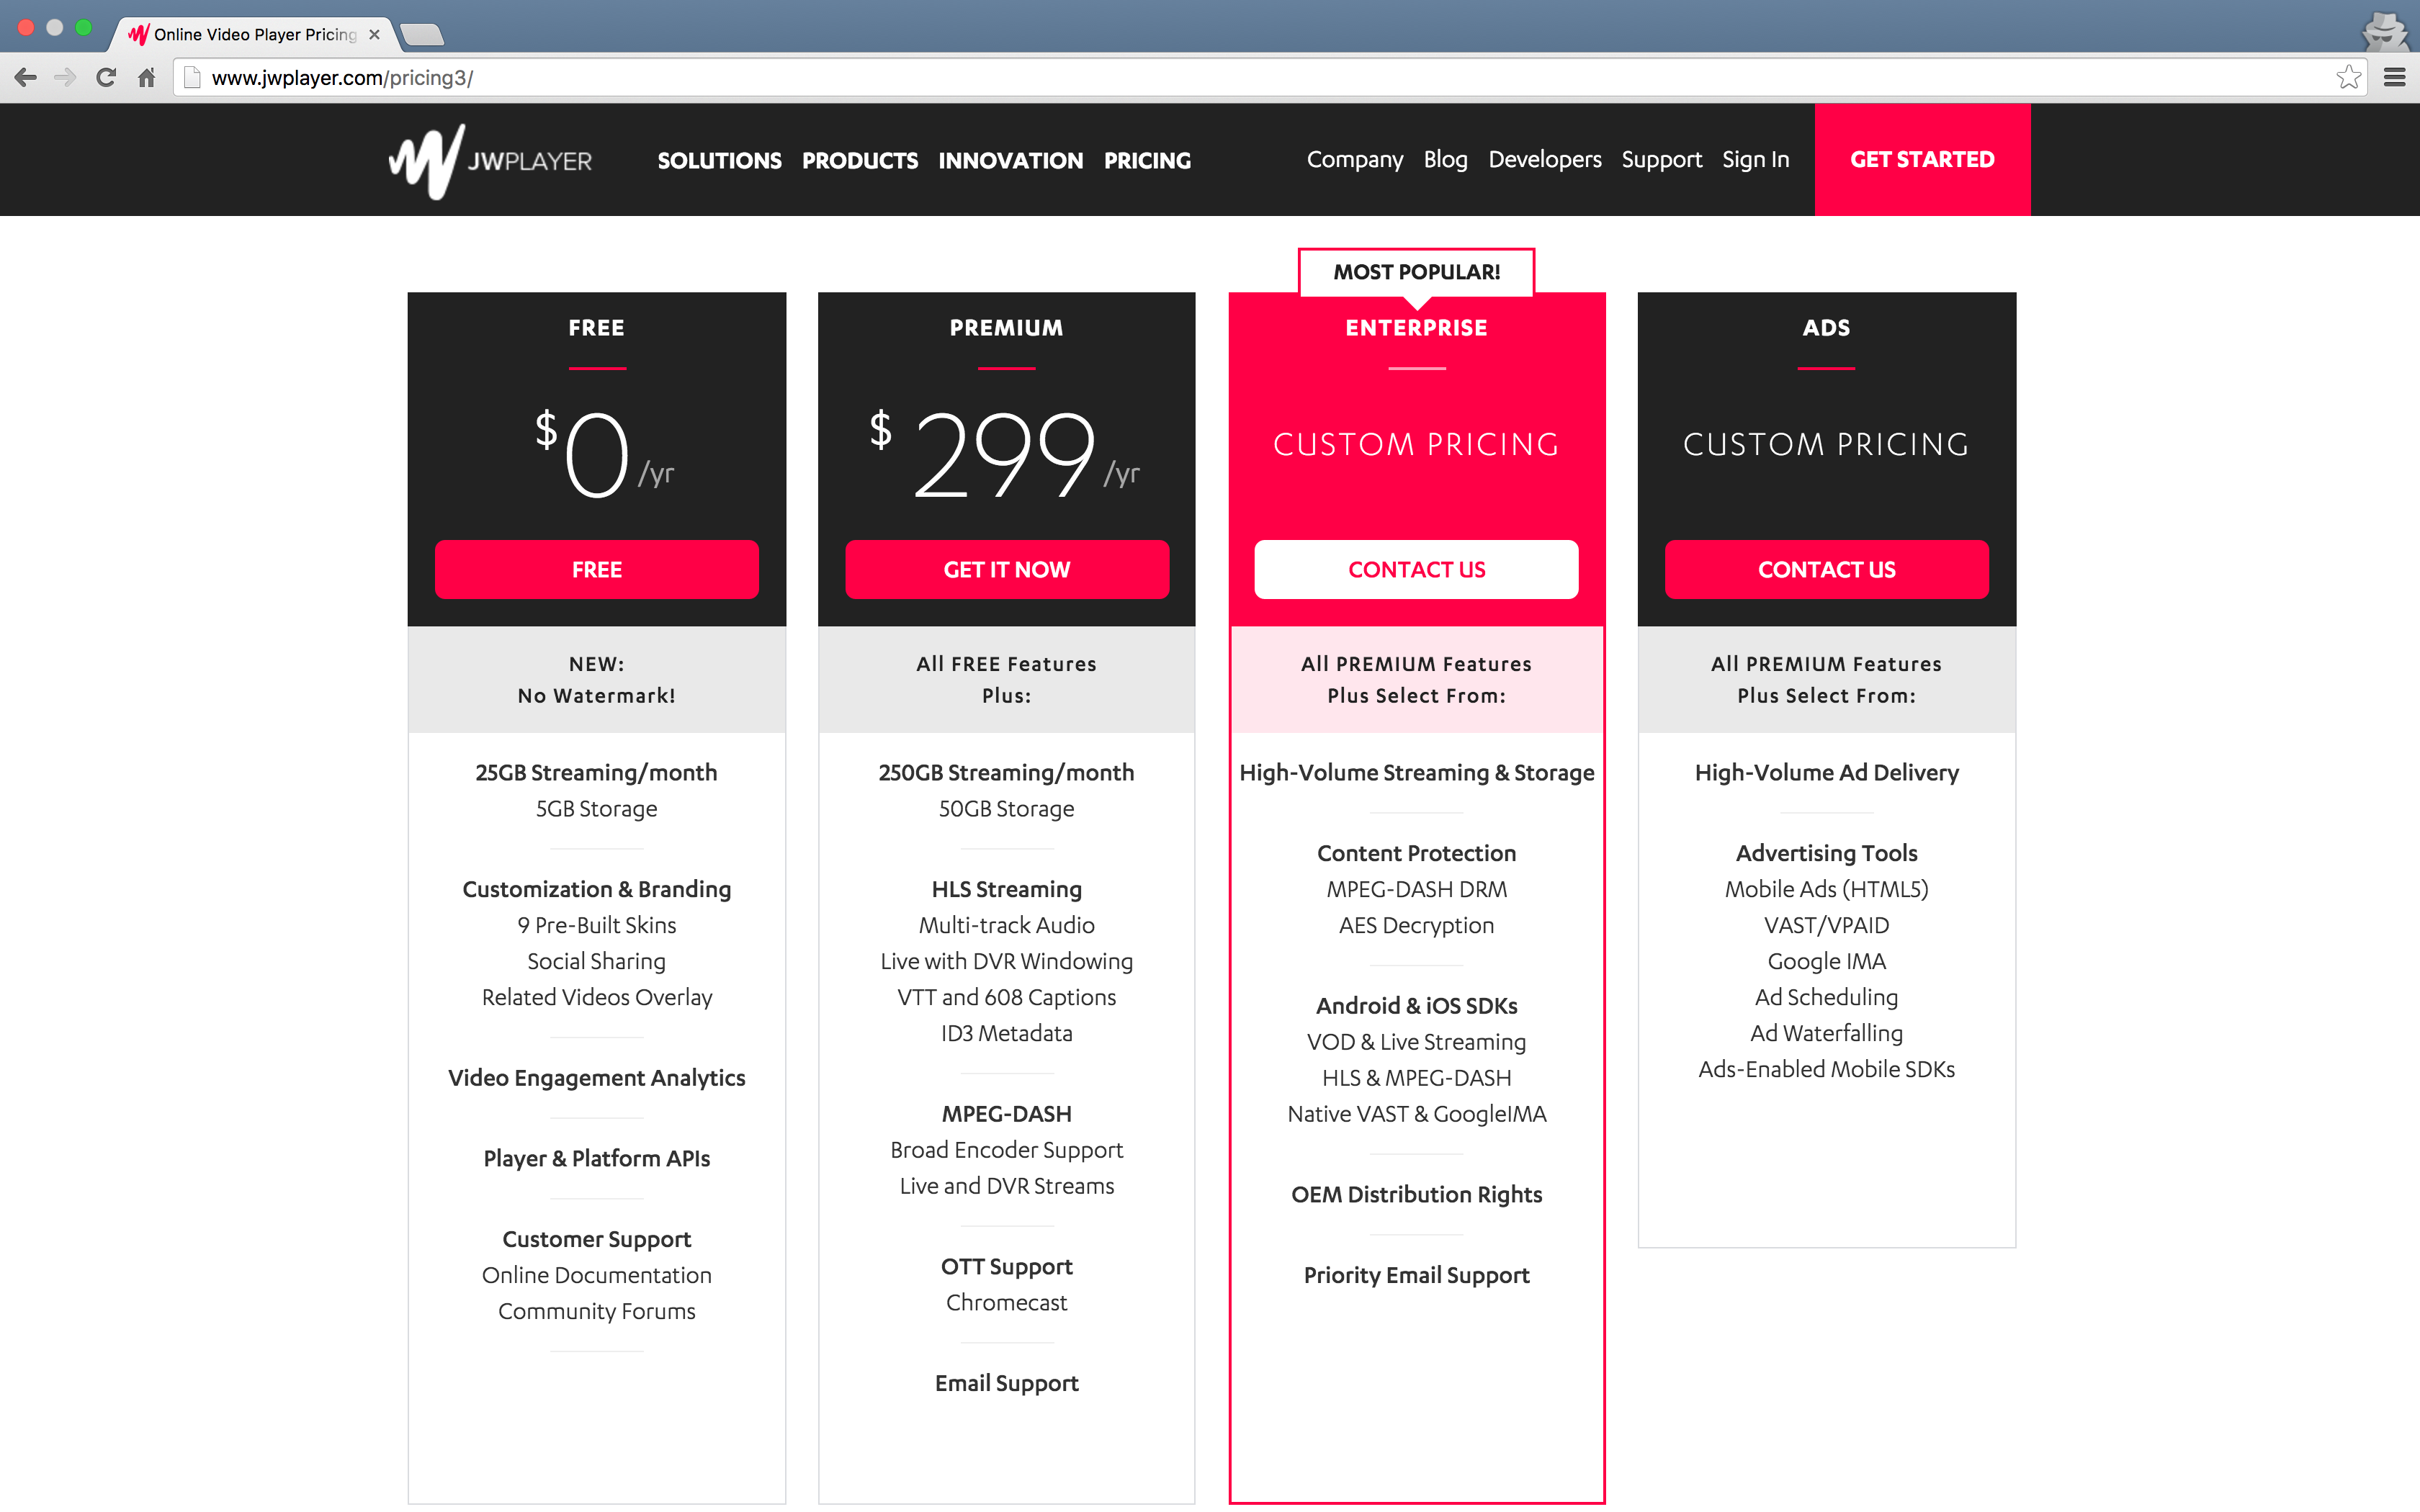
\includegraphics[width=1.0\linewidth]{images/chapter3/jwtPLayer.png}\hfill
 \caption[Web Components]{Web Components}
 \label{fig:fourV}
\end{figure}

